%! TeX root = ./rims-smooth-paper.tex
\documentclass[./rims-smooth-paper.tex]{subfiles}
\begin{document}
\section{Implementation}
\label{sec:impl}
As an implementation language, we adopt a Haskell~\cite{haskell.org:2021tt}, a purely functional lazy programming language.
It has several virtues useful for our purpose:
\begin{enumerate}
\item It supports higher-order functions natively.
\item It is a lazy language, enabling us to treat \emph{infinite} structures.
\item The type-class mechanism in Haskell allows us to use function overloading in handy.
\item Its type system allows us to implement complex inductive types safely.
\end{enumerate}
For a general discussion on the advantages of using Haskell in computer algebra, we refer readers to Ishii~\cite{ISHII:2018ek}.

We follow the standard pattern in implementing ADs in Haskell: we use the function overloading to implement operations on types corresponding ADs.
This strategy is taken, for example, in Karczmarczuk~\cite{Karczmarczuk:2001ww}, Elliott~\cite{Elliott2009-beautiful-differentiation} and implemented in \texttt{ad} package~\cite{Kmett:2010aa}.
In Haskell, the \hask{Floating} type-class gives an abstraction over floating-point numbers that admit elementary functions, as excerpted in \Cref{lst:cls-floating}.
\begin{listing}[tbp]
\begin{code}
class Fractional a => Floating a where
  pi :: a
  exp :: a -> a
  log :: a -> a
  log\base :: a -> a -> a
  sin :: a -> a
  asin :: a -> a
  ...
\end{code}
\caption{The \texttt{Floating} class\label{lst:cls-floating}}
\end{listing}
\begin{listing}[tbp]
\begin{code}
  data AD a = AD a a deriving (Show, Eq, Ord)
  instance Floating a => Floating (AD a) where
    exp (AD f f') = AD (exp f) (f' * exp f)
    sin (AD f f') = AD (sin f) (f' * cos f)
    log (AD f f') = AD (log f) (f' / f)
    ...
\end{code}
\caption{The definition of \texttt{AD}\label{lst:def-AD}}
\end{listing}

For example, a simple forward-mode AD implemented as a dual number can be defined as in \Cref{lst:def-AD}.
The data-type \hask{AD} encapsulates a value of some univariate function and its first-order differential coefficient and calculates the result using the Chain Rule, using \hask{Floating}-operations on the coefficient \hask{a}.

So our goal is to implement \hask{STower n a} data-type conveying information of \emph{all} the higher-order derivatives of an $n$-variate smooth function on \hask{a}, which has \hask{Floating (STower n a)} instances for all \hask{Floating a} and $n$.
In addition, we demand the implementation to be \emph{succinct} and \emph{efficient}, in a sense that it avoids equivalent calculation as much as possible.
For example, if we want to calculate $f_{xy^2}(a,b)$ and $f_{x^2y}(a,b)$ for some smooth $f: \R^2 \to \R$, it should calculate the derivatives up to $f_{xy}$ at most once and share their results in computing both $f_{xy^2}$ and $f_{x^2y}$; in other words, results up to $f_{xy}$ must be \emph{memoised}.

To that end, we employ an infinite tree representation.
The main idea is to use an $n$-ary infinite tree to express a (piecewise) smooth functions: the root node corresponds to the value $f(\boldsymbol{a})$, and its child in the $n$\textsuperscript{th} branch corresponds to $\partial x_n f(\boldsymbol{a})$.
The intuition in the trivariate case is depected in \Cref{fig:tree-simpl}.
\begin{figure}[tbp]
  \centering
  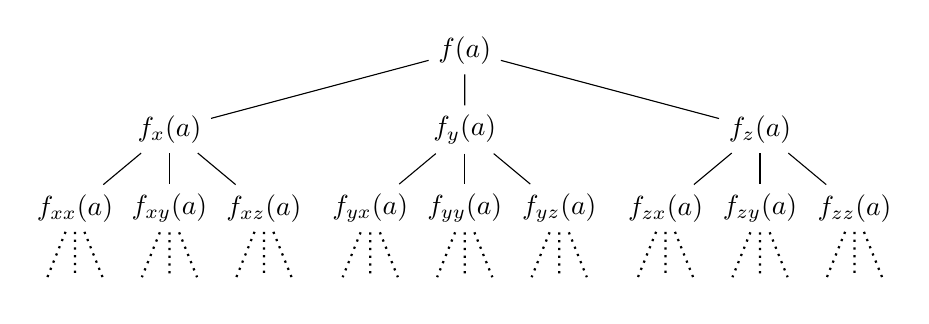
\begin{tikzpicture}[
    level/.style={level distance=1cm},
    level 1/.style={sibling distance=3.75cm},
    level 2/.style={sibling distance=1.2cm},
    level 3/.style={sibling distance=4mm}
    ]
    \newcommand{\ba}{\boldsymbol{a}}
    \node (fa) {$f(\ba)$}
      child{ 
        node (fxa) {$f_x(\ba)$}
          child { 
            node (fxxa) {$f_{xx}(\ba)$}
            child {node{} edge from parent[thick,dotted]}
            child {node{} edge from parent[thick,dotted]}
            child {node{} edge from parent[thick,dotted]}
          }
          child {
            node (fxya) {$f_{xy}(\ba)$}
            child {node{} edge from parent[thick,dotted]}
            child {node{} edge from parent[thick,dotted]} 
            child {node{} edge from parent[thick,dotted]}
          }
          child { 
            node (fxza) {$f_{xz}(\ba)$}
            child {node{} edge from parent[thick,dotted]}
            child {node{} edge from parent[thick,dotted]}
            child {node{} edge from parent[thick,dotted]}
          }
      }
      child {
        node (fya) {$f_y(\ba)$}
        child { 
          node {$f_{yx}(\ba)$} 
          child {node{} edge from parent[thick,dotted]}
          child {node{} edge from parent[thick,dotted]}
          child {node{} edge from parent[thick,dotted]}
        }
        child { 
          node {$f_{yy}(\ba)$}
          child {node{} edge from parent[thick,dotted]}
          child {node{} edge from parent[thick,dotted]}
          child {node{} edge from parent[thick,dotted]}
        }
        child { 
          node {$f_{yz}(\ba)$} 
          child {node{} edge from parent[thick,dotted]}
          child {node{} edge from parent[thick,dotted]}
          child {node{} edge from parent[thick,dotted]}
        }
      }
      child {
        node (fza) {$f_z(\ba)$}
        child {
            node {$f_{zx}(\ba)$}
            child {node{} edge from parent[thick,dotted]}
            child {node{} edge from parent[thick,dotted]}
            child {node{} edge from parent[thick,dotted]}
        }
        child {
          node {$f_{zy}(\ba)$}
          child {node{} edge from parent[thick,dotted]}
          child {node{} edge from parent[thick,dotted]}
          child {node{} edge from parent[thick,dotted]}
        }
        child {
            node {$f_{zz}(\ba)$}
            child {node{} edge from parent[thick,dotted]}
            child {node{} edge from parent[thick,dotted]}
            child {node{} edge from parent[thick,dotted]}
        }
      };
  \end{tikzpicture}
  \caption{Trivariate case, first trial\label{fig:tree-simpl}}
\end{figure}
This can be viewed as a nested trie (or prefix-tree) for memoising functions with $n$-many natural number arguments.
Actually, this representation is isomorphic to the one we can obtain when \hask{Sparse} tower from \texttt{ad} package~\cite{Kmett:2010aa} to the fixed-length vectors.
However, as we assume $f$ to be (piecewise) smooth, there are space for optimisation.
That is, in the above representation, $f_{xy}$ and $f_{yx}$ must almost always coincide except on non-smooth points.
In other words, we can assume partial differential operators to be almost always commutative on inputs.
In many applications, the value on the non-smooth points is negligible and hence we must use more \emph{succinct} representation making use of the commutativity.

The idea is simple: if once one goes down $i$\textsuperscript{th} path, we can only choose $j$\textsuperscript{th} branches for $j \geq i$.
This trick is illustrated in \Cref{fig:tree} for trivariate case.
\begin{figure}[tbp]
  \centering
  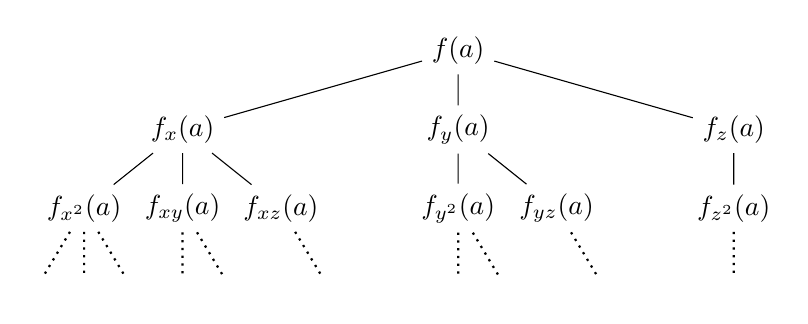
\begin{tikzpicture}[
    level/.style={level distance=1cm},
    level 1/.style={sibling distance=3.5cm},
    level 2/.style={sibling distance=1.25cm},
    level 3/.style={sibling distance=6mm}
    ]
    \newcommand{\ba}{\boldsymbol{a}}
    \node (fa) {$f(\ba)$}
      child{ 
        node (fxa) {$f_x(\ba)$}
          child { 
            node (fxxa) {$f_{x^2}(\ba)$}
            child {node{} edge from parent[thick,dotted]}
            child {node{} edge from parent[thick,dotted]}
            child {node{} edge from parent[thick,dotted]}
          }
          child {
            node (fxya) {$f_{xy}(\ba)$}
            child[missing]
            child {node{} edge from parent[thick,dotted]}
            child {node{} edge from parent[thick,dotted]}
          }
          child { 
            node (fxza) {$f_{xz}(\ba)$}
            child[missing]
            child[missing]
            child { node{} edge from parent[thick,dotted] }
          }
      }
      child {
        node (fya) {$f_y(\ba)$}
        child[missing]
        child { node {$f_{y^2}(\ba)$} child[missing] 
          child {node{} edge from parent[thick,dotted]}
          child { node{} edge from parent[thick,dotted]}
        }
        child { node {$f_{yz}(\ba)$} child[missing] child[missing]
          child {node{} edge from parent[thick,dotted]} }
      }
      child {
        node (fza) {$f_z(\ba)$}
        child {
            node {$f_{z^2}(\ba)$}
            child { node{} edge from parent[thick,dotted] }
        }
      };
  \end{tikzpicture}
  \caption{Trivariate case, succinct version\label{fig:tree}}
\end{figure}
This can be seen as a special kind of an infinite trie (or prefix-tree) of alphabets $\partial_{x_i}$ with available letter eventually decreasing.

We further tweak this representation to make every branching binary (\Cref{fig:tree-tweaked}).
\begin{figure}[tbp]
  \centering
  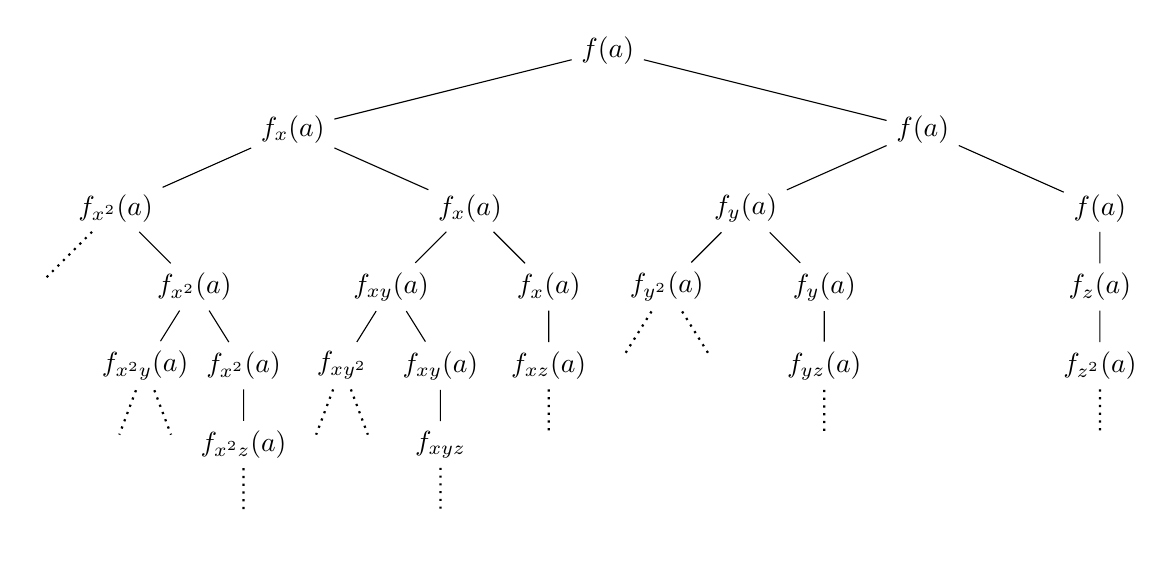
\begin{tikzpicture}[
    level/.style={level distance=1cm},
    level 1/.style={sibling distance=8cm},
    level 2/.style={sibling distance=4.5cm},
    level 3/.style={sibling distance=2cm},
    level 4/.style={sibling distance=1.25cm},
    level 5/.style={sibling distance=0.75cm}
    ]
    \newcommand{\ba}{\boldsymbol{a}}
    \node (fa) {$f(\ba)$}
      child{ 
        node (fxa) {$f_x(\ba)$}
          child { 
            node (fxxa) {$f_{x^2}(\ba)$}
            child {node{} edge from parent[thick,dotted]}
            child {
              node{$f_{x^2}(\ba)$}
              child {
                node {$f_{x^2y}(\ba)$}
                child {node{} edge from parent[thick,dotted]}
                child {node{} edge from parent[thick,dotted]}
              }
              child { node { $f_{x^2}(\ba)$ }
                child { 
                  node { $f_{x^2z}(\ba)$ } 
                  child {node{} edge from parent[thick,dotted]}
                }
              }
            }
          }
          child {
            node {$f_x(\ba)$}
            child {
              node (fxya) {$f_{xy}(\ba)$}
              child {
                node{$f_{xy^2}$}
                child { node{} edge from parent[thick,dotted] }
                child { node{} edge from parent[thick,dotted] }
              }
              child {
                node {$f_{xy}(\ba)$}
                child { 
                  node {$f_{xyz}$}
                  child {node{} edge from parent[thick,dotted]}
                }
              }
            }
            child { 
              node (fxza) {$f_{x}(\ba)$}
              child{
                node {$f_{xz}(\ba)$}
                child {node{} edge from parent[thick,dotted]}
              }
            }
          }
      }
      child
      {
        node {$f(\ba)$}
        child {
          node (fya) {$f_y(\ba)$}
          child { node {$f_{y^2}(\ba)$} 
            child {node{} edge from parent[thick,dotted]}
            child {node{} edge from parent[thick,dotted]}
            }
          child { node {$f_{y}(\ba)$} 
            child {
              node {$f_{yz}(\ba)$}
              child{node{} edge from parent[thick,dotted]}
            }
          }
        }
        child {
          node (fza) {$f(\ba)$}
          child {
              node {$f_{z}(\ba)$}
              child { node {$f_{z^2}(\ba)$}
                child{node{} edge from parent[thick,dotted]}
              }
          }
        }
      }
      ;
  \end{tikzpicture}
  \caption{Trivariate case, tweaked succinct version\label{fig:tree-tweaked}}
\end{figure}
This has two advantages:

\begin{enumerate}
\item We can directly express the tree structure purely as an ADT; we need to use fixed-length vectors here otherwise.\label{item:adt-friendly}
\item Derivatives can be computed simply by induction on the number of variables.\label{item:recurse}
\end{enumerate}

To see these advantages, we now turn to the Haskell implementation (\Cref{lst:data-def}).
\begin{listing}[tbp]
\begin{code}
data STower n a where
  ZS :: !a -> STower 0 a
  SS :: !a -> STower (n + 1) a -> STower n a -> STower (n + 1) a
\end{code}
\caption{Core definitions\label{lst:data-def}}
\end{listing}

\begin{listing}[htbp]
\begin{code}
liftSTower
  :: forall c n a. (KnownNat n, c a, forall x k. c x => c (STower k x) )
  => (forall x. c x => x -> x)
      -- ^ Function
  -> (forall x. c x => x -> x)
      -- ^ its first-order derivative
  -> STower n a
  -> STower n a
liftSTower f df (ZS a) = ZS (f a)
liftSTower f df x@(SS a da dus) = SS (f a) (da * df x) (liftSTower @c f df dus)

instance Num a => Num (STower n a) where
  ZS a + ZS b = SZ (a + b)
  SS f df dus + SS g dg dvs = SS (f + g) (dxf + dxg) (dus + dvs)

  ZS a * ZS b = ZS (a * b)
  SS f df dus * SS g dg dvs = (f * g) (f * dg + df * g) (dus * dvs)

instance Floating a => Floating (STower n a) where
  sin (ZS a) = ZS (sin a)
  sin (SS f df dus) = SS (sin f) (df * cos f) (sin dus)
\end{code}
\caption{Definitions of operations of \texttt{STower}\label{lst:ops-def}}
\end{listing}

\end{document}